\documentclass[10pt,conference]{IEEEtran}
\usepackage{cite}
\usepackage{amsmath,amssymb,amsfonts}
\usepackage{algorithmic}
\usepackage{graphicx}
\usepackage{textcomp}
\usepackage{todonotes}
\usepackage{xcolor}
\usepackage{url}
\makeatletter
\def\endthebibliography{%
	\def\@noitemerr{\@latex@warning{Empty `thebibliography' environment}}%
	\endlist
}
\makeatother
\begin{document}
	
	\title{A Repository for Solidity Smart Contracts\\}
	
	\author{\IEEEauthorblockN{Carl Egge}
		\IEEEauthorblockA{\textit{Institute for Data Engineering} \\
			\textit{Hamburg University of Techology}\\
			Hamburg, Germany \\
			email address or ORCID}
		\and
		\IEEEauthorblockN{Avik Banerjee}
		\IEEEauthorblockA{\textit{Institute for Data Engineering} \\
			\textit{Hamburg University of Technology}\\
			Hamburg, Germany \\
			email address or ORCID}
		\and
		\IEEEauthorblockN{Stefan Schulte}
		\IEEEauthorblockA{\textit{Institute for Data Engineering} \\
			\textit{Hamburg University of Technology}\\
			Hamburg, Germany \\
			email address or ORCID}
		\and
			\IEEEauthorblockN{Michael Schröder}
		\IEEEauthorblockA{\textit{Institute of Information Systems Engineering} \\
			\textit{Technische Universität Wien}\\
			Vienna, Austria \\
			email address or ORCID}
		\and
		\IEEEauthorblockN{Jürgen Cito}
		\IEEEauthorblockA{\textit{Institute of Information Systems Engineering} \\
			\textit{Technische Universität Wien}\\
			Vienna, Austria \\
			email address or ORCID}}
	
	\maketitle
	
	\begin{abstract}
		Blockchain technologies are a growing field of research and public interest. Second generation blockchains, like Ethereum, allow users to execute smart contracts, which are distributed applications executing user-defined logic. This not only expands the utility of blockchains, but also provides new opportunities for tools for solving the same issues that arise with conventional programs. Such tools include optimization of code, detecting code smells and vulnerabilites and developing automated code generation models among others. Such developments require the presence of a dataset of similar code which can be annotated and analyzed according to the desired end application. Existing sources of smart contract code include block explorers that provide limited search and retrieval capabilities on the single version of the contract deployed on the blockchain. Hence to aid the progress of research, this paper introduces the \textit{Smart Contract Repository}---a repository of publicly available Solidity smart contracts, complete with multiple versions of the same contract to help the analysis of the effects of incremental changes in source code.
	\end{abstract}
	
	\begin{IEEEkeywords}
		blockchain, smart contracts, solidity, source code repository
	\end{IEEEkeywords}
	
	\section{Introduction}
	\label{sec:intro}
	Since the introduction of blockchain technologies in 2008~\cite{bitcoinpaper}, the idea to build a completely decentralized Web without firewalls and controlling authorities has gained popularity, leading to the development of applications such as cryptocurrencies and non-fungible tokens ~\cite{crossblockchain}.
	
	First-generation blockchains (e.g., Bitcoin, Litecoin) essentially provide a distributed ledger consisting of append-only blocks, where the trusted central authority is replaced by a network of nodes that share compute power~\cite{blockchainsurvey}. The second generation of blockchains was proposed in 2014 in the Ethereum white paper \cite{ethpaper}, introducing the concept of smart contracts---user-defined pieces of code that reside on the blockchain and are invoked when their accounts are transacted with. Smart contracts are executed in an environment provided by the respective blockchain that is responsible for executing the instructions in the smart contract and taking care of the consequences. The first and the most important example of such an environment is the Ethereum Virtual Machine (EVM) that is responsible for defining and enforcing the rules that govern the computation of a new valid state after the inclusion of a block. The EVM maintains the Ethereum network as a \textit{distributed state machine}, consisting of a state and an associated set of transactions~\cite{wood2019ethereum}. %The structure of the EVM is described in the Ethereum Yellow Paper .
	
	As Ethereum and similar second generation blockchains grow in popularity, the number of deployed smart contracts is growing in number, with the development of newer cryptocurrencies with an emphasis on financial inclusion. Smart contracts provide a way to generate new cryptocurrency tokens, known as \textit{application level tokens} on existing networks without the need to define a new protocol~\cite{commonshood}.\todo{Do we really need this last sentence here? Actually, I think that everything written from ``in number'' is not absolutely necessary, since it does not address the core topics of our work.}
	
	The defining feature of a blockchain is immutability, which makes it very difficult to alter smart contract code that has already been deployed. This raises the need to develop smart contract code that is error-free and efficient before deploying it on the blockchain~\cite{brandstatter}. Deployment and invocation of a smart contract on the blockchain leads to gas fees that are charged to the developer who deploys the smart contract and subsequently to the user who invokes the contract through a transaction~\cite{ethpaper}. This causes each smart contract to have a gas cost associated with it. The gas consumption can, in turn, also estimate the actual energy consumption of the smart contract, since the gas cost is proportional to the computation required for the contract operations~\cite{contractenergyconsumptionthesis}. Thus, it is important to deploy contracts which are error-free and efficient in order to reduce the costs to the user, as also to optimize the energy consumption. 
	
	Source code repositories are an important aid to train systems that identify code smells and vulnerabilities. Code smells  are violations of fundamental design principles in the source code. Code smells can thus, apart from introducing errors in the code, also lead to suboptimal performance and efficiency. Code can further be optimized for maintainability, reusability, comprehensibility and extensibility~\cite{codesmellmining}. Apart from this, versions of the same source code can also provide an insight into the change of performance of the software over consecutive versions\cite{softwareversion}. 
	
	Code mining approaches involve detecting patterns from a repository of source files and analyzing the purpose those patterns serve. Existing code mining approaches mainly involve extracting business logic, automating the translation of code in one language to another, provisioning searching and indexing source files, detecting similarities (used primarily in detecting code smells), to summarize and visualize algorithms and also to extract and analyze information from source code metadata~\cite{codeminingsurvey}.\todo{There is a little bit of a logical gap between this paragraph and the next one. Here, you write about general code mining, in the next about optimization. Try to bridge that gap a little bit.}
	
	However, the principal difference between optimizing conventional programs and smart contracts lies in the fact that smart contracts have to be optimized primarily in terms of the gas cost~\cite{superoptimization}. The smart contract code, when deployed on the Ethereum network, is compiled into \textit{bytecode}. The bytecode is a string made of concatenated op-codes that are executed in sequence when the smart contract is invoked~\cite{wood2019ethereum}. The execution of each opcode is associated with a certain energy consumption, which is calculated and charged from the user according to the EVM \textit{gas model} ~\cite{wood2019ethereum}. This means that optimizing and analyzing smart contracts need to be done not only at the level of the source code, but also at the corresponding bytecode. Optimizing smart contract code directly implies optimizing the gas cost through the bytecode. This introduces an additional constraint and hence requires techniques for constraint-optimized pattern recognition \cite{utilitypattern}.\todo{Since the current version of the repository does not provide the bytecode, do we really want to highlight it here. Also, again, there is a logical/storyline gap between this paragraph and the next one, which should be bridged.}
	
	As already mentioned, consecutive versions of the same source code can help in detecting specific changes to the code performance due to specific changes in the source code ~\cite{softwareversion}. Whereas a comparison between disparate files requires establishment of a similarity measure at the beginning~\cite{simsimilarity}, earlier complete versions of the same source code can provide a benchmark on which to measure the performance of later versions ~\cite{softwareversion}. This can make it easier to detect optimizing patterns in the source code. These patterns, once established, can then be applied to optimizing similar inefficiencies in other source files. Hence, a repository containing multiple versions of each source file would prove to be helpful as a starting point in applying code mining approaches to optimizing smart contracts, which is a relatively unexplored research direction.
	
	Apart from code smell detection and optimization for smart contracts, which is our primary research direction, we believe that this repository can be helpful to researchers in a wide range of other application areas. For instance, code recommendation systems use publicly available code on the Internet to suggest usable pieces of source code to software developers. With the recent progress and development of large language models (LLMs), code generation models such as Codex~\cite{codex} are being used by developers to speed up software design and development, and are proving to be a viable business models for companies. Apart from recommender models focused on source code, general purpose LLMs such as ChatGPT, which is a version of GPT-3 fine-tuned for factoring in human feedback~\cite{chatgpt} also use large datasets of source code in order to make the token embeddings as generalized and diverse as possible~\cite{thestack}. Such models can also be used for code and algorithm summarization and visualization~\cite{codesummarization}. In security research, commits of source code repositories can be used to analyze patterns in smart contract code that eliminate or introduce certain vulnerabilities~\cite{securitydataset}. A dataset of source code can also be used to evaluate and benchmark the performance of static and dynamic analysis tools, which can also be used to detect software vulnerabilities~\cite{staticanalysis}. Analysis of code repositories can also provide useful to generate developer guidelines on writing clean and maintainable code~\cite{maintainablecode}, in the evaluation of software test methods\cite{testmethodevaluation}, in the structural and stylistic comparison of code written in different environments~\cite{codestylecomparison} and in many other studies. \todo{Very fine abstract, showing the need for the work at hand. However, again a logical gap to the next paragraph (i.e., the one about Ethereum).}
	
	The multitude of potential research areas which are based on source code shows the need for the Smart Contract Repository presented in the work at hand.\todo{Please extend this paragraph by writing down what we are actually delivering in this paper.}
	
	Ethereum was the first blockchain to introduce smart contracts and the high-level language Solidity to program smart contracts in. Solidity has grown to be the most mature and popular programming language for smart contracts~\cite{soliditycheck}. A majority of the contracts available on GitHub is written for the Ethereum blockchain, in Solidity~\cite{empiricalgithubcontracts}\todo{I do not see that the referenced paper shows this.}, and hence, Solidity was the language of choice in preparing the dataset\todo{Since it is not described yet what the paper will deliver, the reader actually does NOT know what this ``dataset'' is referring to. If I just read this particular paragraph, I would think that only a dataset is delivered (what we do not do!).}.  The dataset is compiled by crawling through and scraping publicly accessible repositories on GitHub that have Solidity as the main language. The repositories are identified and all available commits of each file are downloaded using the GitHub API. Due to the varying licenses of GitHub repositories, the dataset is being distributed in the form of a Python script which can be run to scrape GitHub and prepare the dataset in an SQLite database. During experimentation, the script collected 163,961 files from 1021 repositories.\todo{I do not like this paragraph too much, since it mixes things up quite a lot. First, it tries to justify why Solidity is used, which is fine (however, better grounding in the literature is necessary). However, afterwards, there is a mixture of repository functionalities and outcomes in terms of the the collected files. Please separate these parts better; this shows also again that it is necessary to first clearly describe what this paper is going to deliver. On another note: I also do not think that the problem with the licenses is highlighted here in enough detail. It's actually mentioned only very very briefly. I do not know if this is taken up later on again, but from I read here, I would not understand (as a normal reader) why there is actually a need for the script at all.}
	
	The remainder of this paper is structured as follows: In Section~\ref{sec:prelims}, we define  prerequisites for our approach. 	Afterwards, Section~\ref{sec:related} discusses the relevant and existing work, Section~\ref{sec:requirements} analyses the requirements for preparing the repository, Section~\ref{sec:implementation} describes how the script\todo{Again, I am not sure if it is too good to write here about the ``script'' alone.} was implemented and how it generates and stores the repository. Finally, Section~\ref{sec:limitations} discusses some limitations of the existing approach and Section~\ref{sec:conclusion} concludes the paper and lays the foundation for future work.
	
	
	\section{Preliminaries}
	\label{sec:prelims}
	
	\subsection{Blockchain:}
	The blockchain technology was introduced by Satoshi Nakamoto in the Bitcoin White Paper \cite{bitcoinpaper}. A blockchain is a tamper-proof distributed ledger, which is similar to a distributed storage of transactions \cite{bitcoinbook} that represent interactions between users. Every transaction is registered in the ledger and the ledger is accessible to all users, thereby making it transparent. The ledger is a chain or immutable blocks which are made tamper-proof using cryptographic techniques. According to Dannen \cite{bitcoinbook}, the blockchain is a combination of the key concepts of Peer-to-peer networking, asymmetric cryptography and cryptographic hashing. Each block in a chain contains a set of transactions along with the hash of the previous block, which links blocks together and makes modification very difficult \cite{bitcoinpaper}. Every block also contains a nonce that is generated along with the block, by solving a hard cryptographic puzzle. This nonce makes it difficult for malicious parties to add blocks to the chain. Transactions are combined into blocks by \textit{miners}.
	
	\subsection{Ethereum:}
	
	While the Bitcoin paper introduced the concept of a blockchain along with a use case in the form of the cryptocurrency Bitcoin, the evolution of blockchains continued after that. In 2013, Vitalik Buterin published the Ethereum White Paper \cite{ethpaper}, which introduced the second generation of blockchains. The Bitcoin protocol only defines the procedure to handle transactions between accounts. Ethereum introduced the ability to run Turing-complete programs on the blockchain, in the form of smart contracts. The technical specifications of Ethereum were spelled out in the Ethereum Yellow Paper \cite{wood2019ethereum}.
	
	With Ethereum, it is theoretically possible to implement and run any kind of service on the blockchain network. In principle, a developer can use any high-level programming language to create an application, compile it to bytecode and deploy it on the blockchain. This allows the program to run on each node in the network and interact with other programs or users on the same network via transactions. In Ethereum, the name Smart Contracts was established for these programs.
	
	\subsection{Smart Contracts}
	In the original Ethereum paper, Buterin described smart contracts as ``systems which automatically move digital assets according to arbitrary pre-specified rules''\todo{I've replaced the quotation marks, but please check how to set them properly in LaTeX (Actually, your IDE shoudl do that for you)}\cite{ethpaper}. A smart contract is a program, that resides on the blockchain and is executed every time a user interacts with it. According to Dannen, smart contracts run business logic and enforce payment agreements between parties \cite{bitcoinbook}. Albert et al. have defined a smart contract from a more technical perspective as a collection of code (its functions) and data (its state) that resides at a specific address on the Ethereum blockchain \cite{gasol}. 
	
	Every smart contract holds pre-defined functions that can be invoked once it is deployed on the blockchain. For instance, a smart contract is created using the constructor method. One can create a contract and take ownership of it by sending a transaction to the constructor method \cite{wood2019ethereum, khanblockchain}. A self-destruct or check-balance function can be generated and used after deployment similarly. Every smart contract has a distinct 20-byte address, is capable of holding an Ether balance, and may respond to incoming transactions using its methods \cite{alharbyblockchain}. It can also be distinguished between deterministic and non-deterministic smart contracts, where deterministic smart contracts do not require any information from outside the blockchain and non-deterministic smart contracts need to access external information (e.g., weather data)\cite{morabito}. Users create and interact with the smart contracts, which are then stored in the blocks on the blockchain. Each smart contract can store code and data that is accessed from the blockchain. The compute power for running the smart contracts is provided by the network itself and the miner nodes that try to append new blocks.
	
	A smart contract can be written in various high-level languages, but is complied into bytecode when deployed on the blockchain. For example, Ethereum introduces the programming language called Solidity, which can used to write smart contracts which are then run on the Ethereum Virtual Machine (EVM). The EVM is a quasi-Turing complete machine \cite{wood2019ethereum} in that it restricts the over-utilisation of resources by limiting the \textit{gas cost}. Each transaction on the Ethereum network has an associated gas consumption, which has to be paid for by the initiator of the transaction. A smart contract is essentially a collection of operations that incur gas cost \cite{wood2019ethereum}. Hence the deployment and invocations of a smart contract have gas consumption associated with them.
	
	The gas consumption of every transaction on the Ethereum chain can be delineated by two properties: \texttt{STARTGAS} and \texttt{GASPRICE}. \texttt{STARTGAS} is the limit of computational steps a contract can execute before it runs out of gas. The \texttt{GASPRICE} is the incentive to miners, per computational step which they carry out. This limitation of gas is essential to prevent smart contracts from going into infinite loops and exponential runtime, which can use up node resources and hence disrupt the entire network \cite{ethpaper}. The Ethereum whitepaper \cite{ethpaper} lists the gas consumption of individual op-codes executed by the Ethereum Virtual Machine (EVM). Reducing the number of such operations and replacing expensive operations with cheaper ones can reduce the gas cost and hence, indirectly, the actual energy consumption of the smart contract~\cite{contractenergyconsumptionthesis}.
	
	\subsection{Code Mining}
	Mining software repositories is the process of finding patterns by analyzing the large corpus of source code available in software repositories \cite{msrllm}. Such patterns depend on the type of end-analysis desired and can point to software development best practices, duplicated vulnerable code or optimizing constructs, among others.
	
	Code mining describes the process of automatic evaluation and optimization of software code. This is usually done with source code in a high-level programming language, but it can also be done with low-level bytecode. Good programming follows certain design principles that can be specific to the language that is used and the application that is built, but at the same time general rules apply to nearly all software projects. Violations of these design principles are called code smells \cite{codesmellmining}. One of the main purposes of code mining is to automatically detect and possibly remove code smells. Different algorithms can be used for code mining, depending on the optimizations that should be achieved.
	
	Fowler et al. were the first to describe the term code smell in their book Refactoring \cite{refactoring}.They defined the term as diagnosing constructs that may indicate that the software needs to be refactored. In their book, they identified 22 code smells and suggest ideas of how to handle these design violations.
	
	As the name suggests, code mining aims to analyze source code using data mining methods. Khatoon et al. describe three mining techniques that are commonly used to identify bugs and code smells while developing software: \textit{Rule Mining Techniques} exploit existing software projects to find some rules that can be applied to the code. \textit{Clone detection} is needed when developers reuse code segments of other developers by just copying them. This often safes time, but it can also introduce incomprehensible errors in the code that need to be found. Lastly, \textit{API usage} is investigated. Calling an external library often requires some checks beforehand or afterwards \cite{khatoon}. In all of these areas, code mining techniques can be used to analyze the source code and improve its quality by finding code smells.
	
	Code mining can therefore include different techniques and tools and is applicable to achieve different goals. Pham et al. find that it can be used “to help understanding, analysing, transforming, improving, maintaining or evolving a particular system, or to improve best practices for the development of new systems” \cite{treemining}. Hence, it is a promising approach to use code mining in the field of gas cost optimization of smart contracts.
	
	\section{Related Work}
	\label{sec:related}
	
	To the best of our knowledge, the analysis of smart contract code has only gained relatively little attention by the research community so far. Nevertheless, there are a number of according approaches for the optimization of gas cost of smart contracts, which we discuss in the following. 
	
	Notably, code smell detection and code optimization for conventional programs have been a very vivid field of research for many years~\cite{codesmellmining} and some of those concepts have trickled down to smart contracts. SmartDagger~\cite{smartdagger} is a tool which uses static analysis of smart contract bytecode to detect cross-contract vulnerability. Manticore~\cite{manticore} is a tool that uses dynamic symbolic execution to test and detect flaws in source code. Existing program verification frameworks such as Boogie or LLVM can be used to perform formal verification of smart contracts~\cite{formalverification}.
	
	
	Brandstätter et al. \cite{brandstatter} explored optimization strategies to implement a rule-based Solidity source code optimizer. The authors conclude that automatic rule detection and optimization need to be extended. Chen et al. have published multiple papers regarding the gas cost optimization of smart contracts \cite{chen1devour, chen2gaschecker, chen3soda, chen4stan}. Starting in 2017, they were one of the first to address the problem of gas optimization. They identified seven antipatterns in Solidity bytecode and presented the tool GASPER to identify three of these gas-costly patterns~\cite{chen1devour}. In 2018, they presented an in-depth investigation and the GasReducer tool, which can automatically check bytecode and run bytecode-to-bytecode optimization for 24 under-optimized code patterns. In 2020, the tools SODA \cite{chen3soda} and GasChecker~\cite{chen2gaschecker} followed, again dedicated to optimize bytecode based on pre-defined rules and patterns. 
	
	Nagele et al. presented the SuperOptimizer \textit{ebso} in 2020. Using techniques of a Satisfiability Modulo Theories (SMT) solver, they developed and tested a tool that can run EVM bytecode optimizations \cite{nagele}. In 2017\todo{As written before, rather do not provide any years/dates in the running text. The exception is the work by Chen et al., since this tells a nice story.. I would not do that for Albert et al., even though they also have two papers. }, Albert et al. presented EthIR, ``a framework for analyzing Ethereum bytecode'' \cite{ethir}. EthIR is an extension of OYENTE that was published by Luu et al. \cite{oyente}. OYENTE is a symbolic execution tool that works with smart contract bytecode and detects bugs for pre-deployment mitigation. It uses the Z3 theorem solver~\cite{z3solver} for symbolic execution of the smart contract code~\cite{oyente}. In 2020, Albert et al. introduced the Eclipse\footnote{Eclipse IDE: https://www.eclipse.org/ide/} plugin GASOL that allows the user to investigate and optimize their Solidity code with different cost models \cite{gasol}.
	
	Most of the published work in the field of optimization of smart contracts focus on the analysis of the compiled bytecode and on detecting similarities between the source code and predefined patterns that can indicate vulnerabilities and malicious constructs. There has been limited research on deriving those patterns from a\todo{Something is wrong here} automatically, which could lead to the automation of existing optimization possibilities while providing opportunities for previously undetected optimization patterns.  Instead, the existing attempts at automating the optimization of smart contracts mainly utilize static and dynamic analysis of the smart contract source code or bytecode\todo{Is this sentence really necessary? It sounds like a little bit of a repetition}.\todo{Logical gap here again: Why is the third paper from Albert et al. mentioned here? The framing is not really good. Or should there be a paragraph before starting with the dicussion of the third Albert et al. paper?} In 2022, Albert et al. published another tool called Syrup~\cite{superoptimization} that is aimed at optimizing smart contracts based on an analysis of the blocks in the Control Flow Graph. The tool breaks up each block into sub-blocks based on state-modifying instructions and sends each sub-block to a Max-SMT solver such as Z3~\cite{z3solver} to obtain an optimized version of the sub-block~\cite{superoptimization}. Feist et al. published Slither, a framework for static analysis of smart contracts. Slither provides information regarding the performance, accuracy and robustness of smart contracts. However, the static analysis is less focused on the gas cost~\cite{slither}. Di Angelo et al. released an investigation and listing of 27 different tools designed to analyze smart contracts \cite{diangelo}. They concluded that the research community was in need of an open source benchmark suite of smart contracts. Chunmiao Li proposed optimization techniques for smart contracts using machine learning and deep learning techniques to estimate the gas consumption of specific types of constructs, such as loops and storage manipulation~\cite{chunmiaoli}. 
	
	As is evident from the previous discussion, a reasonably large repository of smart contracts such as the one presented in this paper is essential, both for deriving new approaches to automatically optimizing smart contracts and for evaluating and benchmarking such tools. Using such a repository combined with static analysis of smart contracts can provide additional patterns that can be used to optimize new contracts, without depending on fixed rules or the optimization capability of SMT solvers.
	
	In the domain of repositories of smart contracts, Pierro et al. developed the Smart-Corpus software that creates a repository of verified smart contracts extracted from Etherscan and allows the download of and computation of metrics on the contracts in the repository~\cite{smartcorpus}. Other repositories, such as the ones by Ren et. al.~\cite{renrepo}, Ferreira et. al.~\cite{ferreirarepo} and SCRAWLD~\cite{scrawld} all contain deployed versions of smart contracts or synthetic smart contracts and do not have associated version histories. The Smart Contract Repository presented in this paper is distinct and novel in that it includes metadata as well as the complete version history of each contract and is not limited to a particular use case. Thus, this repository can prove useful to all use cases mentioned in this section. 
	
	Apart from improving other smart contracts, a repository can also benefits researching conducting\todo{''researching conducting''? Is this correct?} studies on contract design patterns. For example, Wöhrer et al. presented recommendations for the development of smart contracts closely connected to the money transferring fashion of smart contracts~\cite{wohrer}. In 2020\todo{Again, please get rid of the years. This is never done.}, Marchesi et al. presented 24 design patterns for smart contracts categorized based on their features \cite{marchesi}. While most of such studies are based on manual inspection of existing smart contracts, a corpus of smart contracts may be helpful in automating the detection of such patterns and potentially analyzing their effects on gas cost. Additionally, evaluating and designing new programming languages aimed at providing predictable gas consumption with efficient bytecode, requires a dataset of smart contracts\todo{The final sentence is for sure correct, but do you have a reference for this?}.
	
	As mentioned in Section~\ref{sec:intro}, many applications developed for conventional code can be extended to smart contracts with training and evaluation on the proposed dataset.  Recommendation systems such as HelpMeOut~\cite{helpmeout}, ParseWeb~\cite{parseweb} and others could be trained to recommend snippets of Solidity code. LLMs focused on code, such as Codex \cite{codex} could be trained on the repository to work with smart contracts to add to its capabilities. In security research, apart from analysing individual deployed smart contracts, their version histories stored in the repository could be used to detect patterns that introduce or resolve vulnerabilities extending the work done, e.g., in~\cite{securitydataset}. Since the programming languages used in writing smart contracts are high-level languages similar to conventional programming languages, most of the existing tools and research can be extended to smart contracts. A complete repository of source code is the first step in achieving that aim. Our repository aims to fill that gap and provide researchers with complete information regarding smart contract source code and their versions. This repository is different from the repository of smart contracts that can be obtained from existing APIs, such as those provided by Etherscan\footnote{https://etherscan.io/}, since such APIs can only provide a single version of a smart contract deployed on the blockchain.
	\todo{The RW section is in general well-written, but there are some unwanted repetitions. For instance, you should discuss the weaknesses of Etherscan when it is mentioned the first time. Not start discussing it, then do something else, then go back to Etherscan. This is just one example - paper text should have also a high cohesion and loose coupling, just like code.}
	
	
	
	\section{Requirements Analysis}
	\label{sec:requirements}
	As written above, the repository introduced in this paper aims to help researchers and software developers move away from the existing rule-based approaches and derive applicable patterns from analyzing existing source files and versions thereof. Multiple versions of the same source file can be analyzed to find out incremental optimizations to gas consumption and the specific statements or constructs that are behind those optimizations. That is why this repository needs to source its data from publicly available repositories that also store multiple incremental versions of the smart contracts. This can be achieved by crawling repositories that use versioning systems like Git to store commits of the source files.  
	
	As has been described in Section~\ref{sec:intro}, we opted to support Solidity in the repository, since Solidity is the most established programming languages for smart contracts today~\cite{soliditycheck}. We keep the option open to add further languages like Vyper or Yul, if they find a wider distribution in the future. 
	
	In order to follow the best practices for creating a repository, a number of approaches for collecting datasets were studied. One of the best examples of preparing a large scale dataset from GitHub repositories can be found in \cite{thestack}. In the area of smart contracts, repositories can be found in the works of \cite{ren},\todo{Broken reference} \cite{ferreirarepo} and others. Similar to these datasets, our repository should contain the source code of all available contracts. Apart from the source files themselves, additional features need to be incorporated through the storage of metadata about the smart contracts, in order to provide researchers with complete information and to reduce the amount of pre-processing required before analyzing the code in the repository. Also, multiple versions of the source code, if available, can be used to compare incremental changes to the gas consumption and also to detect the introduction to vulnerabilities through changes in the source code. The metadata may include the name of the contract, a description of what it is intended for, details about the source repository, the compiler versions used to generate the bytecodes and also the commit messages, which can be helpful in manual annotation of changes. As mentioned in \cite{thestack}, the repository creation procedure should take into account repository licenses, particularly if the repository is to be made publicly available. The repository should be able to filter out files without permissive licenses.
	
	The repository needs to be stored in a database along with an appropriate database management system (DBMS) that can enable easy and efficient querying capabilities. For this purpose, SQL databases such as SQLite, MySQL or NoSQL databases such as MongoDB can be used.  The smart contracts should be searchable using their metadata, names, the language used, and the corresponding compiler versions. A general purpose relational DBMS or an off-the-shelf document retrieval system operating on a NoSQL database provides ready deep and optimized querying capabilities while ensuring scalability and extendability to newer fields that can be added to the database.
	
	\todo{As discussed today, and also mentioned above: I am clearly missing a discussion of the need for the script. The reviewers will not understand why it is needed. We need a paragraph on this, clearly giving this information.}
	
	\section{Implementation}
	\label{sec:implementation}
	
	The task of generating this repository was completed through the following sub-tasks::
	\begin{itemize}
		\item \textit{Selecting a data source}: Pierro et al. list some sources that can be used to collect smart contract source code from the Web \cite{pierro}. These resources include commonly known code repository hosting platforms (GitHub\footnote{https://github.com}, GitLab\footnote{https://about.gitlab.com} and BitBucket\footnote{https://bitbucket.org}). Additionally, several Ethereum block explorers are available. These services allow for different kinds of interactions with and the analysis of the Ethereum blockchain. EtherScan\footnote{https://etherscan.io/} and EtherChain\footnote{https://etherchain.org/} are two examples of block explorers. In their paper, Pierro et al. use the API of EtherScan to collect verified smart contracts and store them in a database~\cite{pierro}. However, block explorers can only provide the version of the smart contract that is deployed on the blockchain, but not its previous versions. Hence, for the work at hand, GitHub was selected as the source of the data in the repository. GitHub also provides a large volume of source files available and integration with Git, which ensures availability of versions of the source files. Other similar repositories such as GitLab or BitBucket have severely limited or pay-walled provisions for searching and crawling. GitHub, on the other hand, ensures accessibility of the code and its versions through its APIs. GitHub's APIs also allow the user to search for and download files based on the licensing scheme adopted by the developers. This enables the script introduced in this paper to allow users to distinguish between files with viral and non-viral licenses. 
		\item \textit{Automating the data collection process}: To perform data collection from GitHub automatically, a python script was implemented. The script is based on the \textit{github-searcher}\footnote{https://github.com/ipa-lab/github-searcher} written by Schröder et al. to run a stratified search for code snippets on all public repositories~\cite{schroder}. This is done to circumvent the limitation of 5000 requests per hour per API-token imposed by the GitHub API in its free version.
		\item \textit{Collecting the required files}: The implemented script prepares the search by requesting the user for the following information:
		\begin{itemize}
			\item \texttt{database}: the name of an existing database to store the results in. If not provided, the script creates a database file called \texttt{results.db}.
			\item \texttt{statictics}: the name of an existing file to store the search statistics in.
			\item \texttt{min-size}: the minimum file size to search for and collect.
			\item \texttt{max-size}: the maximum file size to search for and collect. GitHub itself imposes a limit of 384 KB on the file size.
			\item \texttt{stratum-size}: the lengths of file-size ranges to be used for the stratified search.
			\item \texttt{no-throttle}: to disable request throttling.
			\item \texttt{search-forks}: this option, if set to \texttt{true}, adds \texttt{fork:true} to the GitHub search query and includes forks of repositories in the search. This expands the field of search but risks including duplicate files in the results.
			\item \texttt{license-filter}: if set to \texttt{true}, filters the search results to include only open-source licensed repositories.
			\item \texttt{github-token}: lets the user enter a GitHub API token in order to access the search APIs. If an API token is present in the environment variables, it is used automatically.
		\end{itemize}
		
		In addition to the restriction of a maximum of 5000 requests per hour, the GitHub search API also imposes a limitation of 1000 results per query. To get around this restriction, the script restricts searches to a certain file size. The script makes use of the technique of \textit{stratified sampling}~\cite{stratifiedsampling}, running the same query, but with different file size ranges in order to retrieve a larger number of files. Further, to download all files returned by the GitHub API, even within the 1000 file limit, the script makes use of \textit{Pagination}~\cite{pagination}, with 100 elements per page.
		
		The sampling statistics file is used to store information about a previously incomplete search, in order to start from the last checkpoint in case of a connection failure, a fatal exception or an interruption by the user. To avoid the secondary rate limit imposed by the GitHub API (to prevent denial of service attacks through a large number of requests from the same source within a short period of time), the script introduces a delay between consecutive calls of the search API. For each file-size range, the query is repeated twice, once in the original order and again in a reverse order, thus sampling the population from both ends, in order to avoid the 1000-results-per-query limit to the best of our ability.
		
		After the required parameters are collected, the script uses the GitHub API to search for repositories that have Solidity as the main language. 
		
		In general, the script performs the following operations to collect data:
		\begin{itemize}
			\item It accesses a list of files for each public repository using the GitHub API\footnote{https://api.github.com/repos/$<$owner$>$/$<$repository$>$/git/trees/master?\\recursive=1}. Searching for Solidity files within this list creates a collection of contract files for each repository. Using the regex \texttt{\textbackslash w\textbackslash .sol} on the file path, the script determines if a file is written in Solidity. For each file, the path and the repository are also stored.
			\item The script accesses a list of commits for each file through the corresponding GitHub API\footnote{ https://api.github.com/repos/$<$owner>/$<$repository$>$/commits?path=\\$<$file\_path$>$}. Iterating through all the files and calling the API for each one creates a version history of each Solidity file, ordered chronologically.
			\item The script downloads the raw source code for each file using the GitHub user content API\footnote{ https://raw.githubusercontent.com/$<$owner$>$/$<$repository$>$/\\$<$commit\_sha$>$/$<$file\_path$>$}.
		\end{itemize}
		
		During experimentation, this resulted in a collection of 163,961 Solidity files, including 299,437 commits. At this point, the script has collected all data it needs to store in the persistent storage to create the repository. All these solidity files have their complete version history and metadata that are the distinctive features of this repository.
		
		The source stored for each file in the repository helps to track modifications to the same file and also files belonging to the same repository or project. However, one drawback of this approach is that forks cannot be filtered and hence can lead to duplicate files in the repository. The \texttt{search-forks} option tries to solve this problem by eliminating fork search altogether. However, a more nuanced comparison of duplicates is required to have the expanded field of search while avoiding duplicates. A hash-based solution (as implemented by the duplicate-file-finder\footnote{https://github.com/michaelkrisper/duplicate-file-finder}) can be adopted to compare files and remove duplicates. 
		
		The collected data are stored in an SQLite database. SQLite was chosen because of its lightweight, cross-platform nature and the absence of the need for any administration. SQLite databases enable the user to analyze the dataset using simple yet powerful command line tools. SQLite interfaces come included with popular programming languages like Python and R, thereby reducing the users' overheads for setting up and maintaining a database. The script introduced in this paper stores all collected information, including the file metadata in three tables:
		\begin{enumerate}
			\item \texttt{REPO}: This table contains information about each collected repository. The schema is as follows:
			\begin{itemize}
				\item \texttt{REPO\_ID INTEGER PRIMARY KEY}: An integer uniquely identifying each collected repository. Acts as the primary key for the table.
				\item \texttt{NAME TEXT NOT NULL}: The name of the repository.
				\item \texttt{FULL\_NAME NOT NULL}: The full name of the repository, including the owner's username.
				\item \texttt{DESCRIPTION TEXT}: A description of the repository from the README.md file.
				\item \texttt{URL TEXT NOT NULL}: The complete URL of the repository.
				\item \texttt{FORK INTEGER NOT NULL}:  The number of forks of the repository.
				\item \texttt{OWNER\_ID INTEGER NOT NULL}: The user ID of the owner.
				\item \texttt{OWNER\_LOGIN}: The username of the owner.
			\end{itemize}
			\item \texttt{FILE}: A table to store the files collected from the \texttt{master} branch of each repository. The schema is as follows:
			\begin{itemize}
				\item \texttt{FILE\_ID INTEGER PRIMARY KEY}: A unique ID for each file.
				\item \texttt{NAME TEXT NOT NULL}: The name of the file.
				\item \texttt{PATH TEXT NOT NULL}: The full path of the file in the GitHub repository.
				\item \texttt{SHA TEXT NOT NULL}: The SHA-1 hash of the latest commit of the file.
				\item \texttt{REPO\_ID INTEGER NOT NULL}: The unique repository ID; references the \texttt{REPO\_ID} from the \texttt{REPO} table.
			\end{itemize}
			\item \texttt{COMMIT}: A table to store the commits for each collected file. This table stores the version history of the files to aid in analyzing incremental changes. The schema is as follows:
			\begin{itemize}
				\item \texttt{COMMIT\_ID INTEGER PRIMARY KEY}: A unique ID assigned to each commit.
				\item \texttt{SHA TEXT NOT NULL}: The SHA-1 hash of the committed file.
				\item \texttt{MESSAGE TEXT NOT NULL}: The commit message.
				\item \texttt{SIZE INTEGER NOT NULL}: The size of the commit in bytes.
				\item \texttt{CREATED DATETIME DEFAULT CURRENT\_TIMESTAMP}: The timestamp of the commit.
				\item \texttt{CONTENT TEXT NOT NULL}: The contents of the committed file. The source code is stored in this field.
				\item \texttt{PARENTS TEXT NOT NULL}: The SHA-1 hash of the commit the current commit is based on.
				\item \texttt{FILE\_ID INTEGER NOT NULL}: The file ID each commit corresponds to. References the \texttt{FILE\_ID} from the \texttt{FILE} table.
			\end{itemize}
			The size, in bytes, of the file content is obtained from the length of the content of the response object. The timestamp is collected directly from the API response.
		\end{enumerate}
		
	\end{itemize}
	
	The repository can be accessed using standard SQLite CLI tools and also through the Python and R interfaces for in depth and automated analysis.
	
	\section{Limitations}
	\label{sec:limitations}
	The script presented in this paper attempts to create a repository of smart contracts, complete with their metadata, source information and most importantly and distinctively, version histories, in order to aid researchers offer a fully functional corpus and provide as much readily available information as possible to perform their aimed analyses. 
	
	The application itself, however, has some limitations with regard to additional functionalities. Though the repository is fully functional, the information stored in the repository can still be enhanced to add even more ready information to the researchers. Each version of a source file can be associated with its corresponding bytecode and ABI, for faster analysis of incremental changes to gas costs. Also the Solidity compiler versions can be retrieved from the file header and stored separately to enable querying for files with specific compiler Solidity versions.
	
	Limitations also arise from the crawling process, the most important one being the fact that the scraping is currently limited to Solidity. Although the data model stores strings and hence can handle any syntax and language, the database has been built with Solidity contracts in mind. However, as discussed before, the script can be extended to include other languages including letting the user decide their language of choice.
	
	It can be argued that a database containing files originating only from public repositories of GitHub may not be representative of the currently deployed smart contracts. As mentioned before, multiple block explorers are available that list deployed smart contracts. However, most of these block explorers do not make the source code of the contracts is publicly accessible, neither do they offer access to multiple versions of the same contract, a limitation which arises from the immutability of the blockchain. Under such circumstances, choosing GitHub is the logical choice since GitHub is the most popular among software development organizations, which makes it easier to assume that the code available on GitHub at least provides an estimation of deployed code. Similar approaches of using GitHub as a source of data for code mining algorithms can be found in literature\cite{schroder, dabic, yang}. However, usage of GitHub can lead to the inclusion of unfinished and untested source code in the repository, and as mentioned before, duplicate code, in the absence of a mechanism to properly handle forks. 
	
	Apart from this, restrictions imposed by the GitHub APIs make it difficult to construct a tree-like version history of a particular source file, given the fact that repositories are structured into branches, each branch having a different set of modifications of a file. 
	
	\section{Analysis of the repository}
	In the previous section, it was mentioned that crawling GitHub might lead to distortions in the dataset. This section presents a short quantitative analysis of a sample of the database generated during experimentation. As written in Section~\ref{sec:implementation}, we were able to generate a corpus of 163,961 Solidity files, which were the results of 299,20437 commits to Github.
	
	Figure~\ref{fig:versions} shows the distribution of the number of versions of the collected files. The absolute frequency of occurrence of the number of versions are represented in the graph. The scale of the Y-axis is logarithmic and the data point at 200 versions included all files that have 200 or more versions, in order to improve the readability of the graph. 132519 out of 163931 or around 80\% of the files have only 2 versions. It is evident that only a few smart contracts include more than 100 versions of the source code. In spite of that 31412 files have multiple versions. This provides a reasonably large dataset for code mining.
	
	\begin{figure}[!h]
		\centering
		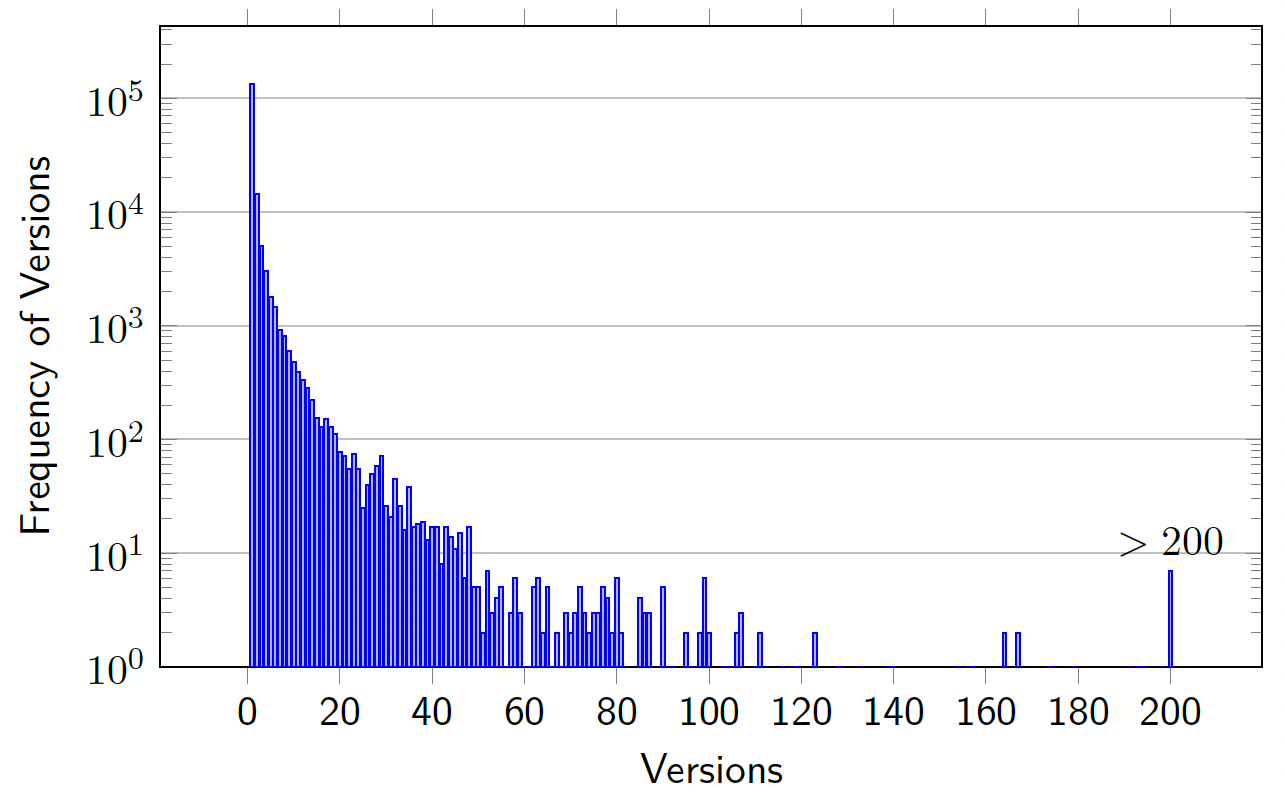
\includegraphics[scale=0.3]{distr_versions_contracts.png}
		\caption{Distribution of versions of smart contracts in the repository}
		\label{fig:versions}
	\end{figure}
	
	When collecting data from GitHub, in the first phase, only the repositories containing Solidity source files were collected. This was followed by scraping all Solidity source files from each of those repositories. This order ensured that all relevant files of each repository were accessed, since the GitHub search API does not return all relevant files by simple content search. As a consequence, all 162931 files in the database come from the same 1021 repositories. To investigate this further, the distribution of files per repository was calculated (see Figure~\ref{fig:number}). This diagram shows the absolute frequency of the number of files that being to a particular repository. The Y-axis is again logarithmic and the data point at 500 includes all repositories having 500 or more relevant files. The repository \textit{ethereum/solidity-fuzzing-corpus} contributed the largest number of files - 33145 - to the repository. 29947 files come from the repository \textit{tintinweb/smart-contract-sanctuary-ethereum}. Additionally, the mean of the distribution is at 160 while the standard deviation is 1514. This shows that a few large repositories have a large impact on the dataset, and consequently, on the quality of source code in it. 13.7\% of the repositories contribute only 3 files. But the high standard deviation captures the widely varying numbers of files contributed by repositories. The outlier of exactly 290 Solidity files that are present in 9 different repositories seems to originate from a specific Solidity tutorial project called \textit{cryptozombies}\footnote{https://cryptozombies.io} that was forked by multiple users on GitHub.
	\begin{figure}[!h]
		\centering
		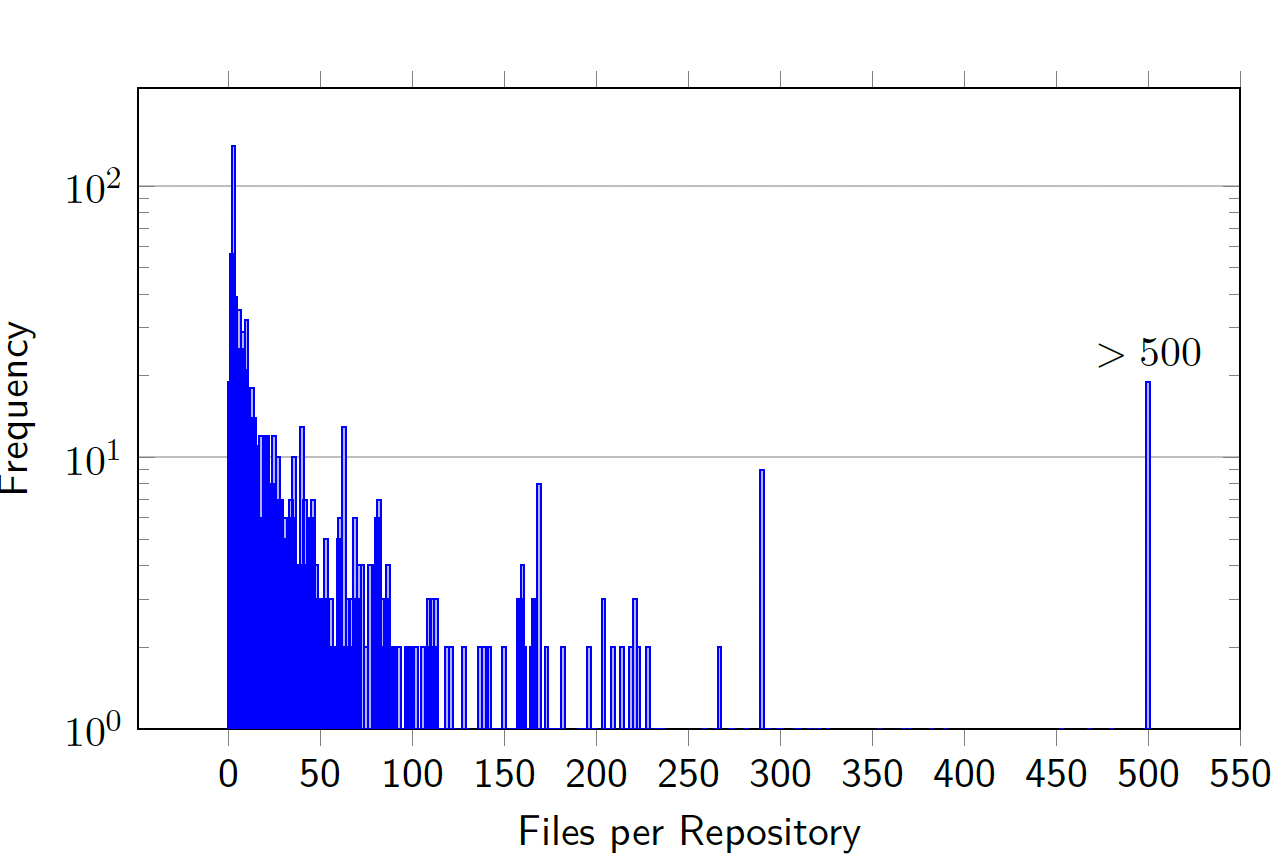
\includegraphics[scale=0.3]{distr_files_repos.png}
		\caption{Distribution of the number of files in the GitHub repositories}
		\label{fig:number}
	\end{figure}
	
	\section{Conclusion}
	\label{sec:conclusion}
	
	Blockchain technologies are a growing industry and research field. With the introduction of smart contracts on second generation blockchains, the scope of application of blockchains has increased, as has corresponding gas costs and consequently, energy consumption. The immutable nature of a blockchain is what makes it secure, but that also means that developers have to write efficient and bug-free code before deploying smart contracts. Hence, tools for developers to optimize and check their code, are under active research. The repository introduced in this paper aims to aid such researchers by helping them to understand and analyze the effects of specific changes of the source code on the outcomes of the smart contract, especially in automating and finding new ways to optimize gas costs. In spite of the mentioned limitations, the repository offers to provide researchers with complete information about a smart contract and its versions.
	
	As has already been mentioned before the script, and consequently the repository, can be extended to include source files using other smart contract programming languages. Also, a compiler can be included as part of the script in order to generate and store the bytecode of the collected contracts. The source of data in the repository can be expanded, crawling other public repositories, or even private repositories a user may have access to. An attempt can be made to reconstruct the version history of a source file across multiple branches of the repository, to enable more fine-grained analysis. A gas-cost estimation framework, such as GASOL \cite{gasol} can be integrated into the script to generate gas cost estimations of the collected contract versions. Finally, the repository can be associated with a Web app that can make it easier to visualize the repository of contracts and also provide APIs for more nuanced filtering and retrieval of the dataset, even without knowledge of SQL. These tools can also be included as a plugin to an IDE that can enable easier interaction with the database.
	
	Apart from the improvements to the repository itself, the next steps involve actually using the repository for applying code mining algorithms, as intended. Upcoming research using this repository should aim at using the enhanced information in this repository towards achieving the research aims mentioned in the previous sections, primarily in the fields of gas consumption, machine learning and qualitative and quantitative analysis of the smart contracts.
	\bibliographystyle{IEEEtran}
	\bibliography{biblio}
	
\end{document}
